\section{Strongly Connected Components}
\subsection{Introduction}
Strongly Connected Components (SCC) are an extension of the concept of connexity for directed graphs.

A strongly connected component is a sub-graph in which there is a (directed) path from each vertex of the component to each vertex of the component.

An example is given in the graph below. There are three strongly connected components.
\begin{center}
  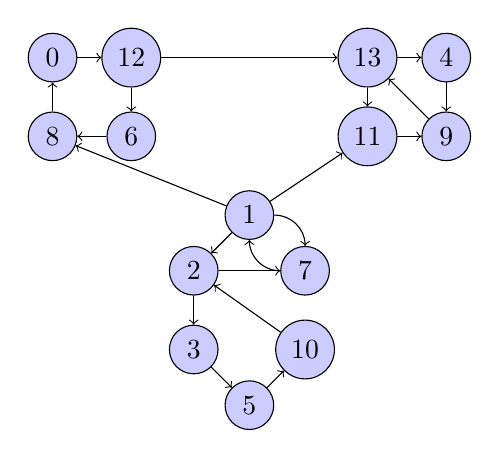
\begin{tikzpicture}[->,nodes={draw, fill=blue!20, circle},row sep=0.3cm,column sep=1cm]
    \node (a0) {0};
    \node (a1) [right of=a0] {12};
	\node (a2) [below of=a1] {6};
    \node (a3) [left of=a2] {8};
    
    \node (b0) [right of=a1,xshift=2cm] {13};
    \node (b1) [right of=b0] {4};
    \node (b2) [below of=b1] {9};
    \node (b3) [left of=b2] {11};
    
    \node (c0) [below of=a3,yshift=-0cm,xshift=2.5cm] {1};
    \node (c1) [below right of=c0] {7};
    \node (c2) [below left of=c0] {2};
    \node (c3) [below of=c1] {10};
    \node (c4) [below of=c2] {3};
    \node (c5) [below right of=c4] {5};
    
    \draw (a0) -> (a1);
    \draw (a1) -> (a2);
    \draw (a2) -> (a3);
    \draw (a3) -> (a0);
    
    \draw (b0) -> (b1);
    \draw (b0) -> (b3);
    \draw (b1) -> (b2);
    \draw (b3) -> (b2);
    \draw (b2) -> (b0);
    
    \draw (c0) -> (c2);
    \draw [->] (c1) to [bend left=45] (c0);
    \draw [->] (c0) to [bend left=45] (c1);
    \draw (c2) -> (c4);
    \draw (c4) -> (c5);
    \draw (c5) -> (c3);
    \draw (c3) -> (c2);
    \draw (c2) -> (c1);
    
    \draw (c0) -> (a3);
    \draw (c0) -> (b3);
    \draw (a1) -> (b0);
  \end{tikzpicture}
\end{center}

\subsection{Properties}
\begin{itemize}
\item Inside a SCC, you are sure that there is a path from everywhere to everywhere;
\item If you contract each SCCs to a single vertex, the resulting graph is a DAG;
\item A transposed graph has the same SCCs as the original one.
\end{itemize}

\subsection{Algorithm}
\subsubsection{Using topological sort}
After having performed the topological sort of the graph, you can use DFS \textbf{using topological order on the transposed graph} to find the SCCs.

The intuition is rather simple: the toposort algorithm on the complete graph will more or less give you the toposort of the DAG of the SCCs; transposing the graph will then allow you to only access the current SCC; each DFS call on a node will give you a new SCC.

\begin{lstlisting}[label=code-scc1,caption=Toposort+DFS, language=Java, tabsize=2, breaklines=true, numbers=left]
void dfsVisit(LinkedList<Integer>[] adj_list, int node, int start_node, int[] labels, Stack<Integer> stack)
{
	labels[node] = OPEN;
	for(int new_node : adj_list[node])
		if(labels[new_node] == UNVISITED)
			dfsVisit(adj_list, new_node, start_node, labels, stack);
	//small change to original DFS: instead of CLOSED, mark nodes as the "start node"
	labels[node] = start_node;
	stack.push(node);
}

LinkedList<Integer>[] transpose(LinkedList<Integer>[] a)
{
	LinkedList<Integer>[] b = new LinkedList[a.length];
	for (int i = 0; i < b.length; i++)
		b[i] = new LinkedList<Integer>();
	for (int i = 0; i < a.length; i++)
		for (int j: a[i])
			b[j].add(i);
	return b;
}

int[] scc(LinkedList<Integer>[] adj_list)
{
	//first, run toposort
	int[] labels = new int[adj_list.length];
	Stack<Integer> stack = new Stack<Integer>();

	Arrays.fill(labels, UNVISITED);
	for(int node = 0; node < adj_list.length; node++)
		if(labels[node] == UNVISITED)
			dfsVisit(adj_list, node, node, labels, stack);

	//run dfsVisit following the toposort order
	labels = new int[adj_list.length];
	LinkedList<Integer>[] adj_list_transposed = transpose(adj_list);
	Arrays.fill(labels, UNVISITED);
	while(!stack.isEmpty())
	{
		int node = stack.pop();
		if(labels[node] == UNVISITED)
			dfsVisit(adj_list_transposed, node, node, labels, stack);
	}

	//Labels now contains the ids of the SCCs.
	return labels;
}
\end{lstlisting}

\subsection{Tarjan's algorithm}
Tarjan's algorithm use a completely different approach, and uses only a single DFS.
It is however less simple to explain, to understand and to use in contests.

\begin{lstlisting}[label=code-scc2,caption=Toposort+DFS, language=Java, tabsize=2, breaklines=true, numbers=left]
int UNVISITED = -1;
int[] dfs_low;
int[] dfs_num;
boolean[] is_in_stack;
Stack<Integer> stack;
int num;
LinkedList< LinkedList<Integer> > sccs;
	
void tarjanVisit(LinkedList<Integer>[] adj_list, int node)
{
	dfs_low[node] = dfs_num[node] = num;
	num++;
	stack.push(node);
	is_in_stack[node] = true;

	for(int s: adj_list[node])
	{
		if(dfs_num[s] == UNVISITED)
		{
			tarjanVisit(adj_list, s);
			dfs_low[node] = Math.min(dfs_low[node], dfs_low[s]);
		}
		else if(is_in_stack[s])
		{
			dfs_low[node] = Math.min(dfs_low[node], dfs_num[s]);
		}
	}
		
	if(dfs_low[node] == dfs_num[node])
	{
		LinkedList<Integer> scc = new LinkedList<Integer>();
		int t;
		do
		{
			t = stack.pop();
			is_in_stack[t] = false;
			scc.add(t);
		} while(t != node);
		sccs.add(scc);
	}
}
	
LinkedList< LinkedList<Integer> > tarjan(LinkedList<Integer>[] adj_list)
{
	dfs_low = new int[adj_list.length];
	dfs_num = new int[adj_list.length];
	is_in_stack = new boolean[adj_list.length];
	stack = new Stack<Integer>();
	num = 0;
	sccs = new LinkedList< LinkedList<Integer> >();
	
	Arrays.fill(dfs_num, UNVISITED);
	Arrays.fill(dfs_low, 0);
	Arrays.fill(is_in_stack, false);
	
	for (int i = 0; i < dfs_num.length; i++) {
		if(dfs_num[i] == UNVISITED)
			tarjanVisit(adj_list, i);
	}
	return sccs;
}
\end{lstlisting}

\subsection{Exercises}

Do the problem 247 from UVA: \url{http://uva.onlinejudge.org/index.php?option=com_onlinejudge&Itemid=8&category=24&page=show_problem&problem=183}